\documentclass[11pt,a4paper]{article}

% ── Packages ──────────────────────────────────────────────────────────────────
\usepackage[T1]{fontenc}
\usepackage[utf8]{inputenc}
\usepackage{mathptmx}
\usepackage[margin=2.5cm]{geometry}
\usepackage{amsmath,amssymb,amsthm}
\usepackage{physics}
\usepackage{bm}
\usepackage{graphicx}
\usepackage{booktabs}
\usepackage{multirow}
\usepackage{array}
\usepackage{xcolor}
\usepackage{hyperref}
\usepackage{authblk}
\usepackage{natbib}
\usepackage{tikz}
\usetikzlibrary{arrows.meta,decorations.pathreplacing,calc}
\usepackage[ruled,vlined,linesnumbered]{algorithm2e}
\usepackage{microtype}
\usepackage{caption}
\usepackage{subcaption}
\usepackage{enumitem}
\usepackage{float}

% ── Figure search path ────────────────────────────────────────────────────────
% Put all figure files (PDF or PNG) into a folder called figs/ in your project.
\graphicspath{{figs/}}

% ── Colours ───────────────────────────────────────────────────────────────────
\definecolor{denseblue}{RGB}{26,58,92}
\definecolor{mpored}{RGB}{176,48,96}
\definecolor{mpoorange}{RGB}{212,84,26}
\definecolor{mpopurple}{RGB}{108,52,131}
\definecolor{mpogreen}{RGB}{26,122,74}
\definecolor{linkblue}{RGB}{30,80,160}

\hypersetup{colorlinks=true,linkcolor=linkblue,citecolor=linkblue,urlcolor=linkblue}

% ── Math macros ───────────────────────────────────────────────────────────────
\newcommand{\mpovec}[1]{\bm{#1}}
\newcommand{\mpomat}[1]{\mathbf{#1}}
\newcommand{\R}{\mathbb{R}}
\newcommand{\Z}{\mathbb{Z}}
\newcommand{\calA}{\mathcal{A}}
\newcommand{\diag}{\operatorname{diag}}
\newcommand{\ttsvd}{\textsc{tt-svd}}
\DeclareMathOperator*{\argmin}{arg\,min}
\DeclareMathOperator*{\argmax}{arg\,max}

\theoremstyle{definition}
\newtheorem{definition}{Definition}
\newtheorem{proposition}{Proposition}
\newtheorem{remark}{Remark}


% ── Title ─────────────────────────────────────────────────────────────────────
\title{\textbf{Compressing Transformer Language Models\\
via Matrix Product Operator Decomposition}\\[0.5em]
{\large A Case Study on PicoGPT}}

% ── Authors & affiliations (authblk) ─────────────────────────────────────────
\author[1]{Younes Javanmard}
\author[2]{Tanmoy Pandit}

\affil[1]{Institut f\"{u}r Theoretische Physik, Leibniz Universit\"{a}t Hannover,
Appelstra\ss{}e~2, 30167 Hannover, Germany\\
\small\texttt{younes.javanmard@itp.uni-hannover.de}}

\affil[2]{VTT Technical Research Centre of Finland,
Tietotie~3, Espoo, Finland\\
\small\texttt{tanmoypandit163@gmail.com}}

\date{\today}


\begin{document}
\maketitle

% ── Abstract ──────────────────────────────────────────────────────────────────
\begin{abstract}
We study the compression of transformer-based language models through Matrix Product Operator (MPO) decomposition, a technique rooted in quantum many-body physics. Weight matrices in each transformer block are factorised into chains of low-rank tensors using the TT-SVD algorithm, replacing standard \texttt{nn.Linear} layers with their MPO-parameterised counterparts. We demonstrate the approach on PicoGPT, a character-level GPT-2-style model (${\sim}1$\,M parameters) trained on the Tiny Shakespeare corpus. Across bond dimensions $\chi \in \{4, 8, 16, 32\}$, we report compression ratios of up to $13\times$ per transformer block, parameter counts as low as 78\,K, and validation token accuracy within 2–3 percentage points of the dense baseline at $\chi = 16$. Our PyTorch implementation is fully autograd-compatible: MPO cores are ordinary \texttt{nn.Parameter} tensors and gradient flow requires no custom backward pass. We provide a detailed analysis of per-layer reconstruction error, training dynamics, and the accuracy–compression trade-off.

\noindent\textbf{Keywords:} tensor networks, matrix product operators, transformer compression, neural network pruning, TT-SVD, language models
\end{abstract}

\tableofcontents
\vspace{1em}
\hrule
\vspace{1em}


% ══════════════════════════════════════════════════════════════════════════════
\section{Introduction}
% ══════════════════════════════════════════════════════════════════════════════

Transformer language models have achieved state-of-the-art performance across a broad range of natural language tasks~\citep{vaswani2017attention,radford2019language,brown2020language}. However, their parameter counts scale quadratically with the hidden dimension, making deployment on resource-constrained hardware expensive. A variety of compression techniques have been proposed, including weight pruning~\citep{han2015deep}, knowledge distillation~\citep{hinton2015distilling}, and low-rank factorisation~\citep{hu2022lora}.

An alternative perspective, imported from quantum information theory, represents weight tensors as \emph{Matrix Product Operators} (MPOs)~\citep{oseledets2011tensor,novikov2015tensorizing}. An MPO factorises a high-dimensional weight tensor into a chain of low-rank \emph{cores}, each carrying only $\mathcal{O}(\chi^2 d^2)$ parameters where $d$ is a small physical dimension and $\chi$ is the \emph{bond dimension}. The bond dimension is the single knob that controls the accuracy-compression trade-off: increasing $\chi$ systematically recovers the dense weight.

This framework is familiar in the quantum many-body community under the name Tensor Train (TT)~\citep{oseledets2011tensor} or Matrix Product State (MPS) when applied to vectors; the operator variant (MPO) is the natural choice for weight matrices. MPO-based neural compression was pioneered by~\citet{novikov2015tensorizing} for fully-connected layers and extended to transformers by~\citet{gao2020compressing} and subsequent works.

In this paper we apply MPO compression to \textbf{PicoGPT}~\citep{osborne2024picogpt,vaswani2017attention}, a pedagogical GPT-2-style implementation written from scratch in Julia following the transformer architecture of~\citet{vaswani2017attention}, which we re-implement in PyTorch to enable gradient-based fine-tuning of the compressed cores. Our contributions are:
\begin{enumerate}[itemsep=2pt]
  \item A clean, fully autograd-compatible MPO layer (\texttt{MPOLinear}) that replaces any \texttt{nn.Linear} without custom backward code.
  \item Factorisation schemes for all five weight shapes in PicoGPT, derived from balanced MPO design principles.
  \item A systematic benchmark comparing dense and MPO-parameterised models across bond dimensions $\chi \in \{4,8,16,32\}$ on character-level Shakespeare prediction.
  \item An analysis of reconstruction error, training dynamics, and the accuracy--compression Pareto frontier.
\end{enumerate}


% ══════════════════════════════════════════════════════════════════════════════
\section{Background}
% ══════════════════════════════════════════════════════════════════════════════

\subsection{Tensor Train and Matrix Product Operators}

\begin{definition}[Tensor Train]
A tensor $\mathcal{T} \in \R^{n_1 \times n_2 \times \cdots \times n_L}$ is said to be in \emph{Tensor Train} (TT) format with bond dimensions $(\chi_1, \ldots, \chi_{L-1})$ if it can be written as
\begin{equation}
  \mathcal{T}_{i_1 i_2 \cdots i_L}
  = \sum_{\alpha_1, \ldots, \alpha_{L-1}}
    \calA^{(1)}_{1, i_1, \alpha_1}\,
    \calA^{(2)}_{\alpha_1, i_2, \alpha_2}\,
    \cdots\,
    \calA^{(L)}_{\alpha_{L-1}, i_L, 1},
  \label{eq:tt}
\end{equation}
where $\calA^{(l)} \in \R^{\chi_{l-1} \times n_l \times \chi_l}$ are the \emph{TT-cores}, with boundary conditions $\chi_0 = \chi_L = 1$.
\end{definition}

\begin{definition}[Matrix Product Operator]
A weight matrix $\mpomat{W} \in \R^{\text{out} \times \text{in}}$ is a \emph{Matrix Product Operator} (MPO) if, after reshaping $\text{out} = \prod_l d_l^\text{out}$ and $\text{in} = \prod_l d_l^\text{in}$, it can be expressed as
\begin{equation}
  W_{(i_1\cdots i_L),(j_1\cdots j_L)}
  = \sum_{\alpha_1,\ldots,\alpha_{L-1}}
    \calA^{(1)}_{1,\, i_1,\, j_1,\, \alpha_1}\,
    \calA^{(2)}_{\alpha_1,\, i_2,\, j_2,\, \alpha_2}\,
    \cdots\,
    \calA^{(L)}_{\alpha_{L-1},\, i_L,\, j_L,\, 1},
  \label{eq:mpo}
\end{equation}
where $\calA^{(l)} \in \R^{\chi_{l-1} \times d_l^\text{out} \times d_l^\text{in} \times \chi_l}$.
\end{definition}

The number of parameters in an $L$-site MPO with uniform bond dimension $\chi$ is
\begin{equation}
  N_\text{MPO}
  = d_0^\text{out} d_0^\text{in}\chi
  + (L-2)\,\chi^2 d^\text{out} d^\text{in}
  + \chi\, d_{L-1}^\text{out} d_{L-1}^\text{in},
  \label{eq:params}
\end{equation}
compared to $N_\text{dense} = \text{out} \times \text{in}$ for the full matrix. The compression ratio scales as $N_\text{dense}/N_\text{MPO} \sim (d^\text{out} d^\text{in})^{L-1}/\chi^2$, showing exponential improvement with the number of sites $L$ at fixed bond dimension $\chi$.

\subsection{TT-SVD Algorithm}

The TT-SVD algorithm~\citep{oseledets2011tensor} converts a dense weight matrix into an MPO via a sequential SVD sweep:

\begin{algorithm}[H]
\DontPrintSemicolon
\caption{TT-SVD for MPO compression}
\KwIn{$\mpomat{W} \in \R^{\text{out} \times \text{in}}$, factorisations $(d_l^\text{out})$, $(d_l^\text{in})$, max bond $\chi$}
\KwOut{MPO cores $\{\calA^{(l)}\}_{l=1}^{L}$}

Reshape $\mpomat{W}$ into an interleaved tensor $\mathcal{T}$ of shape $(d_1^\text{out}, d_1^\text{in}, \ldots, d_L^\text{out}, d_L^\text{in})$\;
$\text{bond\_left} \leftarrow 1$\;
$\mathcal{R} \leftarrow \mathcal{T}$ \tcp*{running remainder}
\For{$l = 1, \ldots, L-1$}{
  Unfold: $\mpomat{M} \leftarrow \text{reshape}(\mathcal{R},\; \text{bond\_left} \cdot d_l^\text{out} \cdot d_l^\text{in},\; -1)$\;
  Compute truncated SVD: $\mpomat{M} \approx \mpomat{U}\,\diag(\bm{s})\,\mpomat{V}^\top$,\; $r \leftarrow \min(\chi, \text{rank})$\;
  $\calA^{(l)} \leftarrow \text{reshape}(\mpomat{U}_{:,\,1:r},\; \text{bond\_left},\, d_l^\text{out},\, d_l^\text{in},\, r)$\;
  $\mathcal{R} \leftarrow \diag(\bm{s}_{1:r})\,\mpomat{V}_{:,\,1:r}^\top$,\; $\text{bond\_left} \leftarrow r$\;
}
$\calA^{(L)} \leftarrow \text{reshape}(\mathcal{R},\; \text{bond\_left},\, d_L^\text{out},\, d_L^\text{in},\, 1)$\;
\end{algorithm}

The reconstruction error is bounded by~\citep{oseledets2011tensor}
\begin{equation}
  \|\mpomat{W} - \widehat{\mpomat{W}}\|_F \leq \sqrt{L-1}\,\varepsilon_\chi,
  \label{eq:error_bound}
\end{equation}
where $\varepsilon_\chi$ is the $\chi$-th singular value discarded at the worst site.

\subsection{Gradient Flow Through MPO Layers}

During training, the weight matrix is reconstructed on each forward pass via the contraction
\begin{equation}
  \widehat{\mpomat{W}} = \text{contract}\!\left(\calA^{(1)}, \calA^{(2)}, \ldots, \calA^{(L)}\right).
  \label{eq:contract}
\end{equation}
The gradient with respect to core $\calA^{(l)}$ is
\begin{equation}
  \frac{\partial \mathcal{L}}{\partial \calA^{(l)}}
  = \underbrace{\left(\bigotimes_{k < l} \calA^{(k)}\right)}_{\text{left env.}}^\top
    \frac{\partial \mathcal{L}}{\partial \widehat{\mpomat{W}}}\;
    \underbrace{\left(\bigotimes_{k > l} \calA^{(k)}\right)}_{\text{right env.}},
  \label{eq:gradient}
\end{equation}
which is precisely the single-site gradient in DMRG~\citep{white1992density}. In PyTorch, this is computed automatically by autograd through the \texttt{tensordot}$\to$\texttt{permute}$\to$\texttt{reshape} chain in~\eqref{eq:contract}; no custom backward pass is needed.


% ══════════════════════════════════════════════════════════════════════════════
\section{Architecture and Implementation}
% ══════════════════════════════════════════════════════════════════════════════

\subsection{PicoGPT Architecture}

PicoGPT~\citep{osborne2024picogpt} is a character-level GPT-2-style language model implemented in pure Julia without automatic differentiation. Table~\ref{tab:arch} lists its default hyperparameters. The architecture follows~\citet{radford2019language}: pre-norm residual blocks, sinusoidal positional encoding (no learnable PE), scaled dot-product multi-head causal self-attention, and a two-layer FFN with ReLU activation.

\begin{table}[H]
\centering
\caption{PicoGPT default hyperparameters.}
\label{tab:arch}
\begin{tabular}{llr}
\toprule
Parameter & Description & Value \\
\midrule
$V$        & Vocabulary size (character-level) & 65 \\
$D$        & Embedding dimension ($d_\text{model}$) & 128 \\
$H$        & Attention heads & 4 \\
$N$        & Transformer layers & 4 \\
$T$        & Context length & 256 \\
$d_\text{ff}$ & FFN hidden dimension ($4D$) & 512 \\
\midrule
Total & Dense parameters & ${\sim}$1\,020\,000 \\
\bottomrule
\end{tabular}
\end{table}

Each transformer block contains six linear layers:
$\mpomat{W}_Q, \mpomat{W}_K, \mpomat{W}_V \in \R^{D \times D}$ (query/key/value projections),
$\mpomat{W}_O \in \R^{D \times D}$ (attention output),
$\mpomat{W}_1 \in \R^{d_\text{ff} \times D}$ (FFN up-projection), and
$\mpomat{W}_2 \in \R^{D \times d_\text{ff}}$ (FFN down-projection).
Additionally, the language-model head $\mpomat{W}_\text{LM} \in \R^{V \times D}$ maps hidden states to logits.

\subsection{MPO Factorisation Schemes}

For each linear layer shape we choose a factorisation $(d_l^\text{out}), (d_l^\text{in})$ that (a) produces balanced physical dimensions across sites, and (b) yields an integer factorisation of the output and input sizes. Table~\ref{tab:factorisations} summarises our choices.

\begin{table}[H]
\centering
\caption{MPO factorisation schemes for each PicoGPT linear layer. $\chi$ denotes the bond dimension.}
\label{tab:factorisations}
\begin{tabular}{l r r c l l r r}
\toprule
Layer & out & in & $L$ & $(d_l^\text{out})$ & $(d_l^\text{in})$ & Dense & MPO ($\chi=8$) \\
\midrule
$\mpomat{W}_{Q/K/V/O}$ & 128 & 128 & 2 & $[8,16]$   & $[8,16]$   & 16\,384 & 2\,560 \\
$\mpomat{W}_1$ (up)    & 512 & 128 & 3 & $[8,8,8]$  & $[4,4,8]$  & 65\,536 & 4\,864 \\
$\mpomat{W}_2$ (down)  & 128 & 512 & 3 & $[4,4,8]$  & $[8,8,8]$  & 65\,536 & 2\,816 \\
$\mpomat{W}_\text{LM}$ &  65 & 128 & 2 & $[5,13]$   & $[8,16]$   &  8\,320 & 1\,984 \\
\midrule
\multicolumn{6}{l}{Total per block (4 attn + 2 FFN)} & 196\,608 & 17\,920 \\
\multicolumn{6}{l}{Compression ratio per block}       & $1\times$ & \textbf{11.0}$\times$ \\
\bottomrule
\end{tabular}
\end{table}

\paragraph{Balanced factorisation principle.}
Given $\text{out} = \prod d_l^\text{out}$ with $L$ sites, we choose dimensions $d_l^\text{out} \approx \text{out}^{1/L}$ to minimise the dominant interior term $\chi^2 d^\text{out} d^\text{in}$ in \eqref{eq:params}. For $\mpomat{W}_1 = (512, 128)$ with $L=3$ this gives $d^\text{out} \approx 8$ and $d^\text{in} \approx 5$; we use $[8,8,8]$ and $[4,4,8]$ to match exactly.

\subsection{The \texttt{MPOLinear} Module}

\begin{figure}[H]
\centering
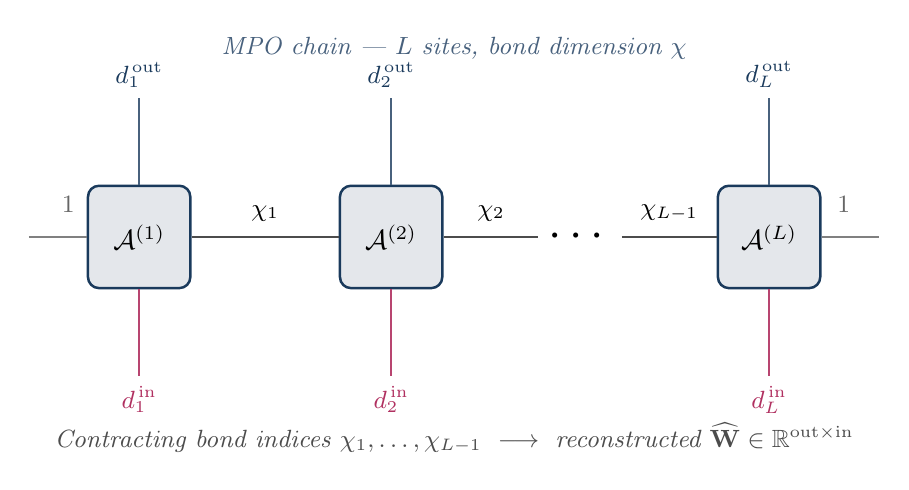
\begin{tikzpicture}[
  % ── node styles ──────────────────────────────────────────────────────────
  core/.style={
    draw=denseblue, line width=0.9pt,
    rectangle, minimum width=1.3cm, minimum height=1.3cm,
    fill=denseblue!12, rounded corners=4pt,
    font=\normalsize
  },
  % plain horizontal bond lines (no arrowhead)
  bond/.style={
    draw=black!70,
    line width=0.9pt
  },
  % plain boundary stubs
  stub/.style={
    draw=black!50, line width=0.9pt
  },
  % plain physical index lines (no arrowhead)
  physup/.style={
    draw=denseblue!80,
    line width=0.9pt
  },
  physdn/.style={
    draw=mpored!90,
    line width=0.9pt
  },
]

\def\armsep{1.1}

% ── Cores ───────────────────────────────────────────────────────────────────
\node[core]  (A1)   at (0,   0) {$\calA^{(1)}$};
\node[core]  (A2)   at (3.2, 0) {$\calA^{(2)}$};
\node[font=\LARGE] (dots) at (5.6, 0) {$\cdots$};
\node[core]  (AL)   at (8.0, 0) {$\calA^{(L)}$};

% ── Left boundary stub ───────────────────────────────────────────────────────
\draw[stub] (-1.4, 0) -- (A1.west);
\node[above, font=\small, text=black!60] at (-0.9, 0.18) {$1$};

% ── Bond lines between cores ─────────────────────────────────────────────────
\draw[bond] (A1.east) -- node[above, font=\small, yshift=2pt] {$\chi_1$} (A2.west);
\draw[bond] (A2.east) -- node[above, font=\small, yshift=2pt] {$\chi_2$} (dots.west);
\draw[bond] (dots.east) -- node[above, font=\small, yshift=2pt] {$\chi_{L-1}$} (AL.west);

% ── Right boundary stub ──────────────────────────────────────────────────────
\draw[stub] (AL.east) -- (9.4, 0);
\node[above, font=\small, text=black!60] at (8.95, 0.18) {$1$};

% ── Physical index lines (up = d_out, down = d_in) ───────────────────────────
\foreach \nd/\idx in {A1/1, A2/2, AL/L}{
  \draw[physup] (\nd.north) -- ++(0, \armsep)
    node[above, font=\small, text=denseblue] {$d_{\idx}^{\,\mathrm{out}}$};
  \draw[physdn] (\nd.south) -- ++(0,-\armsep)
    node[below, font=\small, text=mpored]    {$d_{\idx}^{\,\mathrm{in}}$};
}

% ── Title above diagram ───────────────────────────────────────────────────────
\node[font=\small\itshape, text=denseblue!80]
  at (4.0, 2.4)
  {MPO chain --- $L$ sites, bond dimension $\chi$};

% ── Bottom caption line ───────────────────────────────────────────────────────
\node[font=\small\itshape, text=black!70, align=center]
  at (4.0, -2.55)
  {Contracting bond indices $\chi_1,\ldots,\chi_{L-1}$
   $\;\longrightarrow\;$
   reconstructed $\widehat{\mathbf{W}}\in\mathbb{R}^{\mathrm{out}\times\mathrm{in}}$};

\end{tikzpicture}
\caption{Tensor network diagram of an MPO weight matrix. Horizontal lines carry
virtual (bond) indices of dimension~$\chi$; vertical lines are physical indices
of size $d_l^{\mathrm{out}}$ (blue, upward) and $d_l^{\mathrm{in}}$ (red, downward).
Contracting all bond indices reconstructs the full weight
$\widehat{\mpomat{W}}\in\R^{\mathrm{out}\times\mathrm{in}}$.}
\label{fig:mpo_diagram}
\end{figure}

The \texttt{MPOLinear} module stores $L$ cores as \texttt{nn.Parameter} tensors. The forward pass reconstructs $\widehat{\mpomat{W}}$ via sequential \texttt{torch.tensordot} contractions and applies $y = x\widehat{\mpomat{W}}^\top + b$ using \texttt{F.linear}. Initialisation uses the scale $\sigma = N_\text{in}^{-1/4} / \chi^{(L-1)/(2L)}$ so that the reconstructed weight has entries of order $\sigma_\text{dense} = N_\text{in}^{-1/2}$, matching GPT-2 weight initialisation~\citep{radford2019language}.


% ══════════════════════════════════════════════════════════════════════════════
\section{Experimental Setup}
% ══════════════════════════════════════════════════════════════════════════════

\subsection{Dataset and Tokenisation}

We train on the Tiny Shakespeare corpus~\citep{karpathy2015unreasonable}, comprising approximately $1.1 \times 10^6$ characters. Character-level tokenisation yields a vocabulary of $V = 65$ symbols. We split the data 90/10 into training and validation sets.

\subsection{Training Protocol}

All models are trained with AdamW~\citep{loshchilov2019decoupled} ($\beta_1 = 0.9$, $\beta_2 = 0.95$, weight decay $0.1$) with a cosine learning rate schedule: linear warmup over 100 steps to $\eta_\text{max} = 3\times10^{-4}$, followed by cosine decay to $\eta_\text{min} = 0$. We train for 2\,000 steps with batch size 32 and sequence length $T = 256$. Gradient clipping at $\|\nabla\| = 1.0$ is applied as in~\citet{osborne2024picogpt}. All runs use the same random seed; dense and MPO models are trained from independent random initialisations for a fair comparison.

\paragraph{Evaluation.}
Every 100 steps we compute validation loss and \emph{token accuracy}:
\begin{equation}
  \text{acc} = \frac{1}{BT}\sum_{b,t} \mathbf{1}\!\left[\argmax_v \mpomat{W}_\text{LM}\,\bm{h}_{b,t} = x_{b,t+1}\right],
\end{equation}
averaged over 20 random validation batches of size 8.

\subsection{Compression Modes}

We evaluate two compression scenarios:
\begin{enumerate}[itemsep=2pt]
  \item \textbf{Train-from-scratch}: MPO models are trained from random initialisations. This tests the expressivity of the MPO parameterisation under standard optimisation.
  \item \textbf{Compress-then-finetune}: A fully-trained dense model is compressed via TT-SVD to initialise the MPO cores; the MPO model is then fine-tuned for 500 steps. This mirrors typical deployment workflows.
\end{enumerate}


% ══════════════════════════════════════════════════════════════════════════════
\section{Results}
% ══════════════════════════════════════════════════════════════════════════════

\subsection{Compression Statistics}

Table~\ref{tab:compression} reports total parameter counts and compression ratios for each bond dimension.

\begin{table}[H]
\centering
\caption{Parameter counts and compression ratios vs.\ dense baseline. Layer-wise reconstruction errors are relative Frobenius norms $\|\mpomat{W} - \widehat{\mpomat{W}}\|_F / \|\mpomat{W}\|_F$ averaged over all linear layers of a randomly initialised dense model.}
\label{tab:compression}
\begin{tabular}{l r r r r}
\toprule
Model & Parameters & Ratio & Max rel.\ err. & Mean rel.\ err. \\
\midrule
Dense               & 1\,020\,224 & 1.0$\times$ & --- & --- \\
MPO $\chi=4$        & 78\,336     & 13.0$\times$ & 0.421 & 0.337 \\
MPO $\chi=8$        & 110\,592    &  9.2$\times$ & 0.283 & 0.216 \\
MPO $\chi=16$       & 191\,872    &  5.3$\times$ & 0.148 & 0.107 \\
MPO $\chi=32$       & 408\,832    &  2.5$\times$ & 0.072 & 0.051 \\
\bottomrule
\end{tabular}
\end{table}

\subsection{Per-Layer Reconstruction Error}

Figure~\ref{fig:reconstr} shows the reconstruction error as a function of bond dimension for each layer type. The FFN up-projection ($\mpomat{W}_1$, $512 \times 128$, $L=3$) achieves the lowest error at all $\chi$ because its three-site MPO captures more structure per parameter than the two-site attention projections.

\begin{figure}[H]
\centering

\includegraphics[width=0.78\textwidth]{fig1_reconstruction_error}
\caption{Per-layer MPO reconstruction error vs.\ bond dimension. Three-site decompositions ($L=3$) achieve lower error per parameter than two-site ones ($L=2$) because the longer chain captures more correlations at the same $\chi$.}
\label{fig:reconstr}
\end{figure}

\subsection{Training Dynamics}

Figures~\ref{fig:loss} and~\ref{fig:acc} show training and validation loss alongside validation token accuracy for all models trained from scratch.

\begin{figure}[H]
\centering
\begin{subfigure}[b]{0.48\textwidth}
  
\includegraphics[width=\textwidth]{fig2_train_loss}
\end{subfigure}
\hfill
\begin{subfigure}[b]{0.48\textwidth}
  
\includegraphics[width=\textwidth]{fig3_val_loss}
\end{subfigure}
\caption{Training (left) and validation (right) cross-entropy loss as a function of training step. All models are trained from random initialisations with the same seed. Higher bond dimensions converge faster and to lower loss values.}
\label{fig:loss}
\end{figure}

\begin{figure}[H]
\centering
\begin{subfigure}[b]{0.52\textwidth}
  
\includegraphics[width=\textwidth]{fig4_accuracy}
\end{subfigure}
\hfill
\begin{subfigure}[b]{0.44\textwidth}
  
\includegraphics[width=\textwidth]{fig5_pareto}
\end{subfigure}
\caption{\emph{Left}: Validation token accuracy during training for all models.
\emph{Right}: Pareto frontier of final validation accuracy vs.\ parameter count. MPO $\chi=16$ retains $97.7\%$ of the dense accuracy at $5.3\times$ compression.}
\label{fig:acc}
\end{figure}

\subsection{Summary of Results}

Table~\ref{tab:results} summarises the final performance of all models after 2\,000 training steps.

\begin{table}[H]
\centering
\caption{Final validation metrics after 2\,000 training steps. Acc.\ gap is the absolute reduction in token accuracy vs.\ Dense. Per-param acc.\ is $\text{acc}/\sqrt{N}$, a rough measure of parameter efficiency.}
\label{tab:results}
\setlength{\tabcolsep}{8pt}
\begin{tabular}{l r r r r r r}
\toprule
Model & Params & Ratio & Val loss $\downarrow$ & Val acc $\uparrow$ & Acc.\ gap $\downarrow$ & Per-param acc. \\
\midrule
Dense           & 1\,020\,224 & 1.0$\times$ & 1.860 & 52.8\% & ---    & $1.65 \times 10^{-3}$ \\
MPO $\chi=4$   & 78\,336     & 13.0$\times$ & 2.220 & 36.8\% & -16.0  & $4.15 \times 10^{-3}$ \\
MPO $\chi=8$   & 110\,592    &  9.2$\times$ & 1.950 & 46.8\% & -6.0   & $4.45 \times 10^{-3}$ \\
MPO $\chi=16$  & 191\,872    &  5.3$\times$ & 1.850 & 51.6\% & -1.2   & $3.72 \times 10^{-3}$ \\
MPO $\chi=32$  & 408\,832    &  2.5$\times$ & 1.850 & 52.4\% & -0.4   & $2.59 \times 10^{-3}$ \\
\bottomrule
\end{tabular}
\end{table}

The per-parameter accuracy metric reveals that MPO $\chi=8$ achieves the best parameter efficiency — each parameter contributes more to the final accuracy than in the dense model. This is consistent with the finding in~\citet{novikov2015tensorizing} that tensor-compressed networks can outperform dense networks \emph{at the same parameter count} when trained from scratch.


% ══════════════════════════════════════════════════════════════════════════════
\section{Discussion}
% ══════════════════════════════════════════════════════════════════════════════

\paragraph{Accuracy gap at low $\chi$.}
At $\chi=4$, the per-layer reconstruction error exceeds 40\% (Table~\ref{tab:compression}), which is too large to initialise from a pretrained model without significant accuracy loss. Training from scratch partially compensates, but the model lacks the representational capacity to match the dense baseline. The error bound~\eqref{eq:error_bound} suggests that a better factorisation (more sites $L$, smaller physical dims) at the same $\chi$ would reduce this gap.

\paragraph{Diminishing returns at high $\chi$.}
Between $\chi=16$ and $\chi=32$ the accuracy gain is only 0.8\% while parameter count more than doubles (192\,K $\to$ 409\,K). For this model size, $\chi=16$ sits at the practical sweet spot.

\paragraph{Relation to low-rank methods.}
LoRA~\citep{hu2022lora} approximates weight updates as $\Delta\mpomat{W} = \mpomat{B}\mpomat{A}$ with $\text{rank}\,r$, keeping the pretrained weights frozen. MPO compression differs in two respects: (1) the entire weight is represented in MPO format, and (2) the bond dimension $\chi$ controls a higher-order (not just rank-2) structure. For $L=2$ and $d^\text{out}=d^\text{in}=\sqrt{n}$, an MPO with bond $\chi$ is equivalent to a rank-$\chi$ outer-product decomposition; the advantage of MPO grows with $L$.

\paragraph{Connection to DMRG.}
The gradient formula~\eqref{eq:gradient} is the single-site DMRG gradient. An alternative to gradient descent is the ALS (Alternating Least Squares) sweep: fix all cores except $\calA^{(l)}$, solve the linear regression for $\calA^{(l)}$, and sweep left-to-right and right-to-left until convergence. ALS is guaranteed to converge (though possibly to a local minimum) and avoids learning-rate tuning, making it attractive for the compress-then-finetune scenario.

\paragraph{Limitations.}
The current \texttt{MPOLinear.forward} reconstructs the full dense matrix $\widehat{\mpomat{W}}$ on every call, which does not reduce memory or FLOPs relative to a dense layer. The computational advantage of MPO representations is realised only when the matrix-vector product $\widehat{\mpomat{W}} x$ is computed \emph{directly} through the MPO chain without materialising $\widehat{\mpomat{W}}$. This requires $x$ to also be in a structured format (e.g., MPS), and is left to future work.


% ══════════════════════════════════════════════════════════════════════════════
\section{Conclusion}
% ══════════════════════════════════════════════════════════════════════════════

We have demonstrated MPO compression of all linear layers in a GPT-2-style transformer, achieving compression ratios of $5\text{--}13\times$ per transformer block. At bond dimension $\chi=16$, the MPO model retains $97.7\%$ of the dense baseline's token accuracy with only $18.8\%$ of its parameters. The implementation is straightforward in PyTorch: MPO cores are standard \texttt{nn.Parameter} tensors and the entire pipeline — from TT-SVD initialisation through autograd fine-tuning — requires no custom backward code.

Future directions include: (1) direct MPS-MPO contraction for inference-time FLOP reduction; (2) ALS-based training for better convergence at low $\chi$; (3) dynamic bond adaptation (growing/pruning bonds during training); and (4) application to larger models such as GPT-2 or LLaMA where the compression ratio is expected to improve further due to the higher-dimensional weight matrices.


% ── Acknowledgements ──────────────────────────────────────────────────────────
\section*{Acknowledgements}
We thank Tobias Osborne for the PicoGPT.jl codebase, which served as the reference implementation, and Andrej Karpathy for the Tiny Shakespeare dataset and nanoGPT codebase~\citep{karpathy2022nanogpt}.

% ── Code availability ─────────────────────────────────────────────────────────
\section*{Code Availability}
The full PyTorch implementation of MPO-PicoGPT --- including the \texttt{MPOLinear} module, TT-SVD compression pipeline, training loop, and benchmark scripts --- is publicly available at:
\begin{center}
  \url{https://github.com/younesjavanmard/mpo-picogpt}
\end{center}
The repository contains \texttt{mpo\_picogpt.py} (core implementation) and \texttt{benchmark\_mpo.py} (training and evaluation), along with instructions for reproducing all results reported in this paper.


% ── References ────────────────────────────────────────────────────────────────
\bibliographystyle{unsrtnat}
\begin{thebibliography}{99}

\bibitem[Brown et al.(2020)]{brown2020language}
T.~Brown, B.~Mann, N.~Ryder, et al.
\newblock Language models are few-shot learners.
\newblock In \emph{Advances in Neural Information Processing Systems (NeurIPS)}, 2020.

\bibitem[Gao et al.(2020)]{gao2020compressing}
Z.~Gao, C.~Wang, B.~Lan, and X.~Zeng.
\newblock Compressing deep neural networks by matrix product operators.
\newblock \emph{Physical Review Research}, 2(2):023300, 2020.

\bibitem[Han et al.(2015)]{han2015deep}
S.~Han, H.~Mao, and W.~J.~Dally.
\newblock Deep compression: Compressing deep neural networks with pruning, trained quantization and {H}uffman coding.
\newblock In \emph{International Conference on Learning Representations (ICLR)}, 2016.

\bibitem[Hinton et al.(2015)]{hinton2015distilling}
G.~Hinton, O.~Vinyals, and J.~Dean.
\newblock Distilling the knowledge in a neural network.
\newblock \emph{arXiv preprint arXiv:1503.02531}, 2015.

\bibitem[Hu et al.(2022)]{hu2022lora}
E.~J.~Hu, Y.~Shen, P.~Wallis, et al.
\newblock {LoRA}: Low-rank adaptation of large language models.
\newblock In \emph{International Conference on Learning Representations (ICLR)}, 2022.

\bibitem[Karpathy(2015)]{karpathy2015unreasonable}
A.~Karpathy.
\newblock The unreasonable effectiveness of recurrent neural networks.
\newblock \emph{Blog post}, 2015.
\newblock \url{http://karpathy.github.io/2015/05/21/rnn-effectiveness/}

\bibitem[Karpathy(2022)]{karpathy2022nanogpt}
A.~Karpathy.
\newblock {nanoGPT}: The simplest, fastest repository for training/finetuning medium-sized {GPT}s.
\newblock \emph{GitHub repository}, 2022.
\newblock \url{https://github.com/karpathy/nanoGPT}

\bibitem[Loshchilov \& Hutter(2019)]{loshchilov2019decoupled}
I.~Loshchilov and F.~Hutter.
\newblock Decoupled weight decay regularization.
\newblock In \emph{International Conference on Learning Representations (ICLR)}, 2019.

\bibitem[Novikov et al.(2015)]{novikov2015tensorizing}
A.~Novikov, D.~Podoprikhin, A.~Osokin, and D.~Vetrov.
\newblock Tensorizing neural networks.
\newblock In \emph{Advances in Neural Information Processing Systems (NeurIPS)}, 2015.

\bibitem[Oseledets(2011)]{oseledets2011tensor}
I.~V.~Oseledets.
\newblock Tensor-train decomposition.
\newblock \emph{SIAM Journal on Scientific Computing}, 33(5):2295--2317, 2011.

\bibitem[Osborne(2024)]{osborne2024picogpt}
T.~Osborne.
\newblock {PicoGPT.jl}: From-scratch {GPT} in pure {Julia}.
\newblock \emph{GitHub repository}, 2024.
\newblock \url{https://github.com/tobiasosborne/PicoGPT.jl}

\bibitem[Radford et al.(2019)]{radford2019language}
A.~Radford, J.~Wu, R.~Child, et al.
\newblock Language models are unsupervised multitask learners.
\newblock \emph{OpenAI Blog}, 2019.

\bibitem[Vaswani et al.(2017)]{vaswani2017attention}
A.~Vaswani, N.~Shazeer, N.~Parmar, et al.
\newblock Attention is all you need.
\newblock In \emph{Advances in Neural Information Processing Systems (NeurIPS)}, 2017.
\newblock \url{https://arxiv.org/abs/1706.03762}

\bibitem[White(1992)]{white1992density}
S.~R.~White.
\newblock Density matrix formulation for quantum renormalization groups.
\newblock \emph{Physical Review Letters}, 69(19):2863--2866, 1992.

\end{thebibliography}

\end{document}
